\documentclass[justified]{tufte-handout}
\usepackage{../braph2_tut}
\usepackage{tcolorbox}
%\geometry{showframe} % display margins for debugging page layout

\title{Group of Subjects with Connectivity-Functional Multiplex Data}

\begin{document}

\maketitle

\begin{abstract}
\noindent
For \emph{connectivity-functional multiplex data}, we will upload two folders, one containing the connectivity data and the other functional data for different subjects, that belong to the same group. For example, the connectivity matrix could correspond to white matter tracts obtained from dMRI or pre-calculated coactivations maps obtained from fMRI data, and the functional values could correspond to brain activation signals derived from functional MRI data at different frequencies or time windows. This Tutorial explains how to prepare and work with this kind of data.
\end{abstract}

\tableofcontents

\fig{figure}
	{fig:01}
	{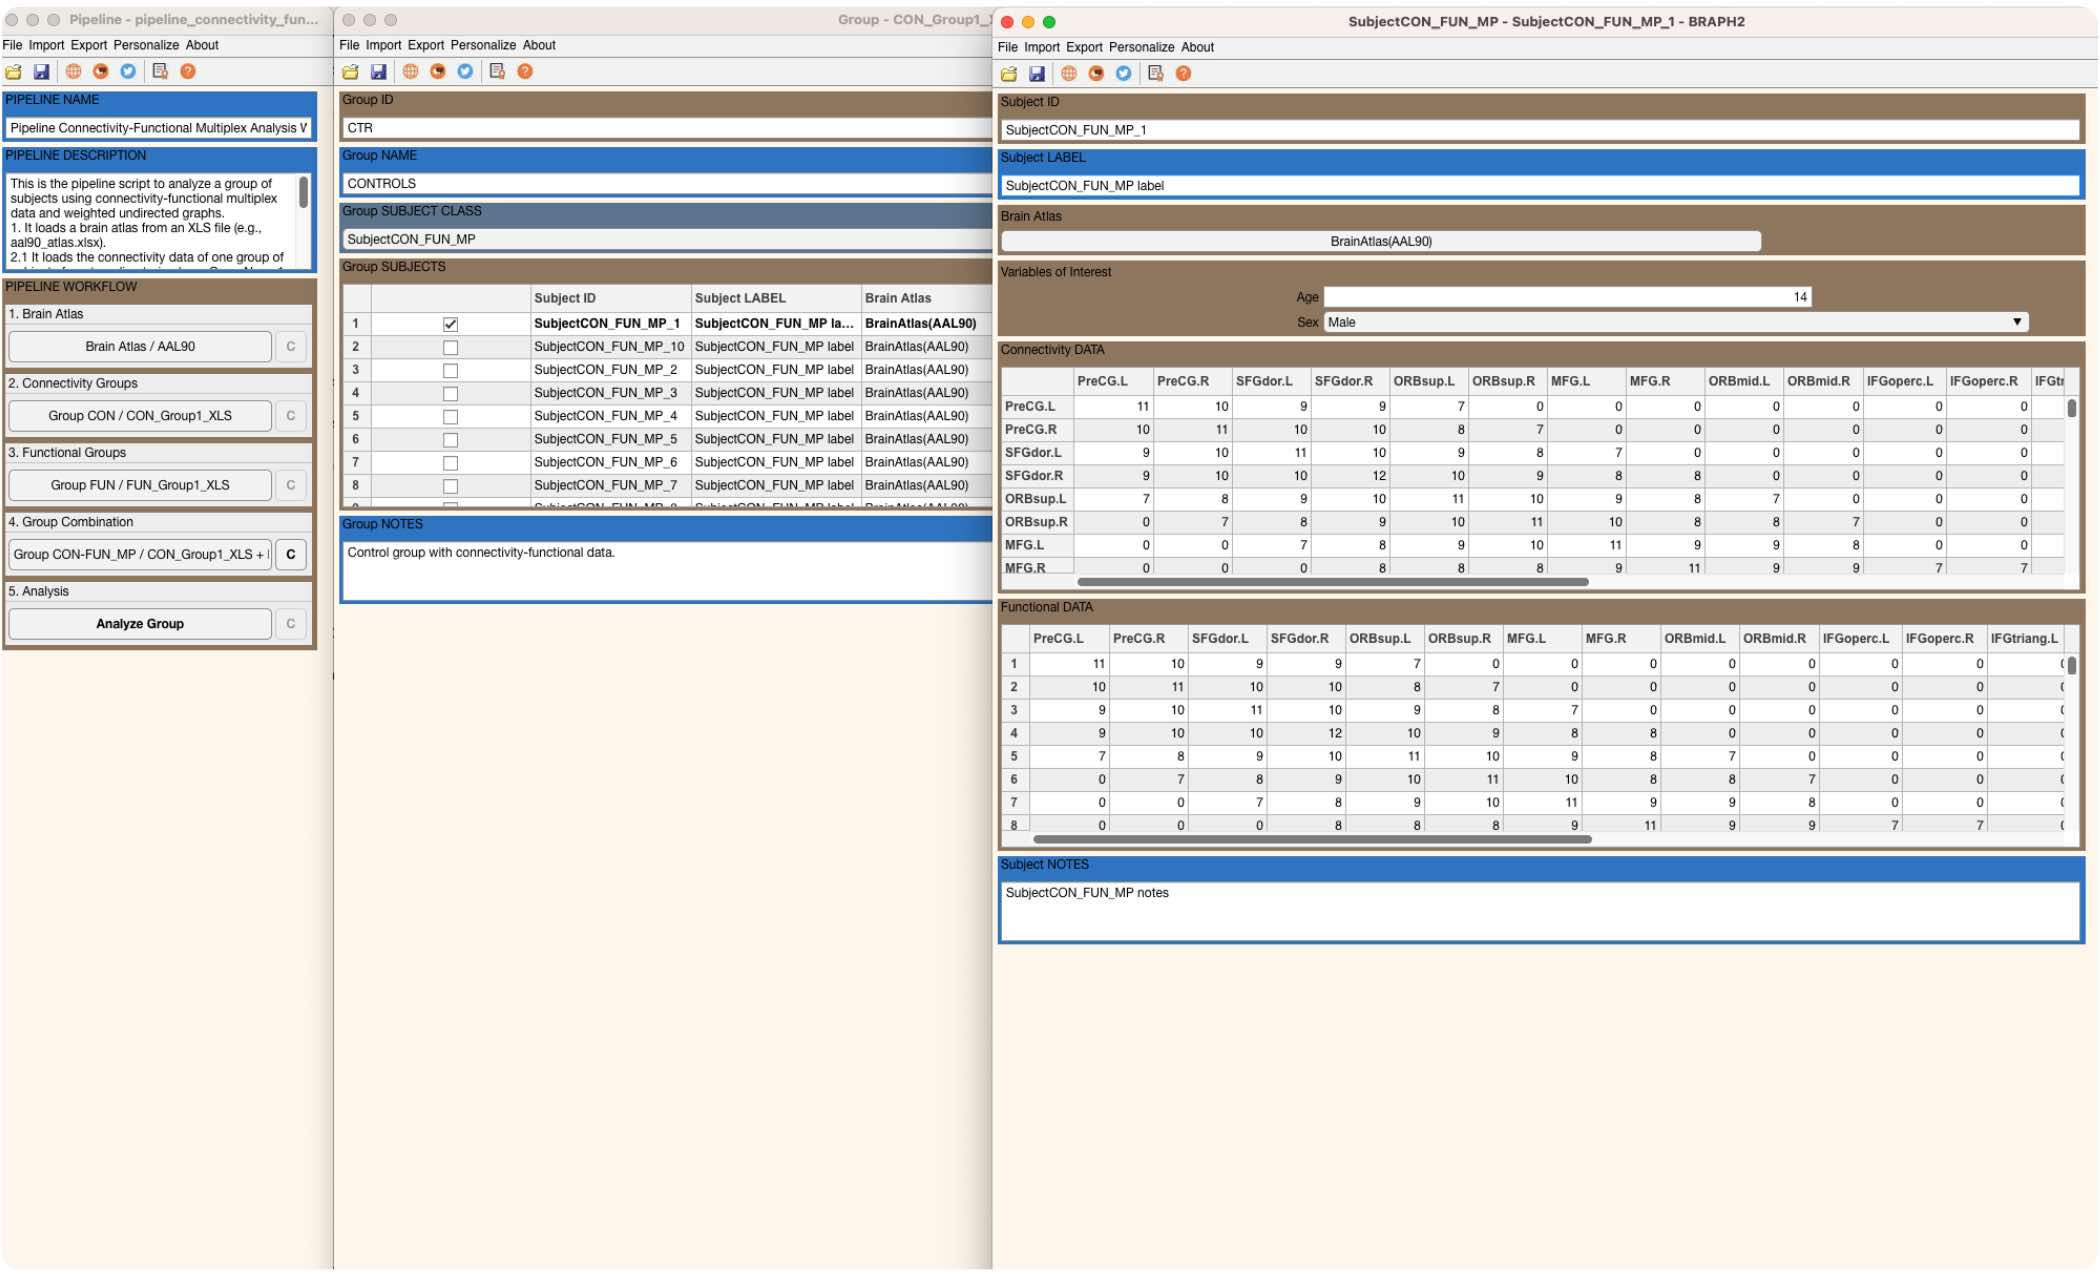
\includegraphics{fig01.jpg}}
	{GUI for a group of subjects with connectivity-functional multiplex data}
	{
	Full graphical user interface to upload a group of subjects with connectivity-functional multiplex data in BRAPH~2.0. 
	}
#!FIG01

\clearpage
\section{Generation of Example Data}

If you don't have the \fn{Example data CON\_FUN\_MP XLS} folder inside \fn{connectivity-functional multiplex}, then you can generate it by running the commands in \Coderef{cd:exampledata}.

\begin{lstlisting}[
	label=cd:exampledata,
	caption={
		{\bf Code to generate the example data folder.}
		This code can be used in the MatLab command line to generate the \fn{Example data CON$\_$FUN$\_$MP XLS} folder to the \fn{connectivity-functional multiplex} pipeline folder.
	}
]
test_CombineGroups_CON_FUN_MP ¥\circled{1}\circlednote{1}{generates the example connectivity-functional multiplex XLS data folder.}¥
\end{lstlisting}

\section{Upload the Group Data}

The second step after you have selected a brain atlas is to upload the group data. You can open an analysis or comparison by typing \code{braph2} in MatLab's terminal, which allows you to select a pipeline containing the steps required to perform your analysis and upload a brain atlas. After these steps have been completed you can upload your group's data. First, you need to upload the connectivity data for a group by clicking ``Load Group CON from XLS'' (\Figref{fig:02}a). After that, you can upload the functional data for the same group by clicking ``Load Group FUN from XLS'' (\Figref{fig:02}b). Finally, press ``Combine Groups'' in order to create a group of subjects with connectivity-functional multiplex data (\Figref{fig:02}c).

\fig{figure}
	{fig:02}
	{
	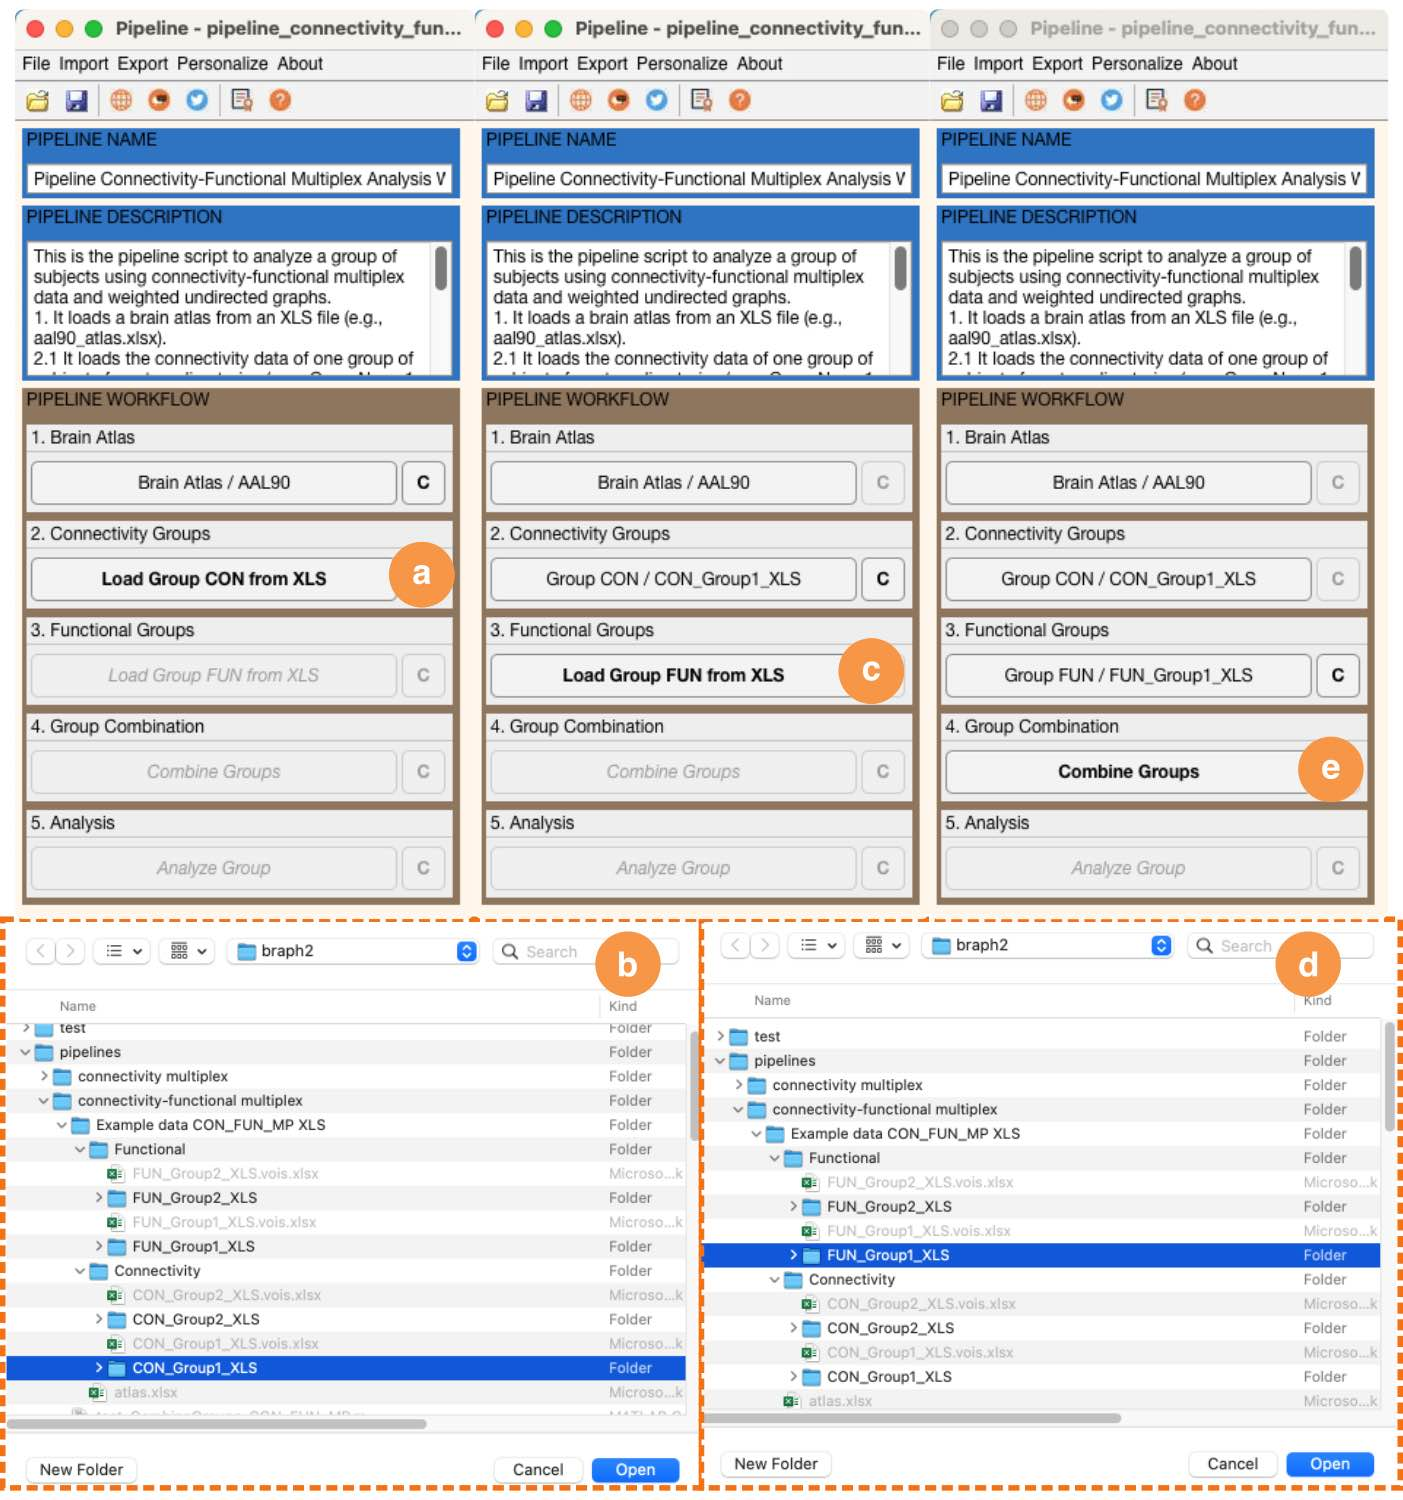
\includegraphics{fig02.jpg}
	}
	{Upload the data of a group of subjects}
	{
	Steps to upload a group of subjects with connectivity-functional multiplex data using the GUI and an example dataset: 
	{\bf a} Upload the connectivity data for a group.
	{\bf b} Import a folder that contains one file per subject with the connectivity matrix in XLS. Here we use the example data: navigate to the BRAPH~2.0 folder \fn{pipelines}, \fn{connectivity-functional multiplex},  \fn{Example data CON\_FUN\_MP XLS}, \fn{Connectivity}, and select the folder containing the connectivity matrices of one group \fn{CON\_Group1\_XLS}.
     {\bf c} Upload the functional data for a group.
 	{\bf d} Import a folder that contains one file per subject with the functional time series in XLS. Here we use the example data: navigate to the BRAPH~2.0 folder \fn{pipelines}, \fn{connectivity-functional multiplex},  \fn{Example data CON\_FUN\_MP XLS}, \fn{Functional}, and select the folder containing the functional data of one group \fn{FUN\_Group1\_XLS}.
   {\bf e} Finally, combine the groups to create a group with connectivity-functional multiplex data.
	}
#!FIG02

\section{Visualize the Group Data}

After completing the steps described in \Figref{fig:02}, you can see the data (\Figref{fig:03}a), and change the Group ID, name, and notes (\Figref{fig:03}b). 

\fig{figure}
	{fig:03}
	{
	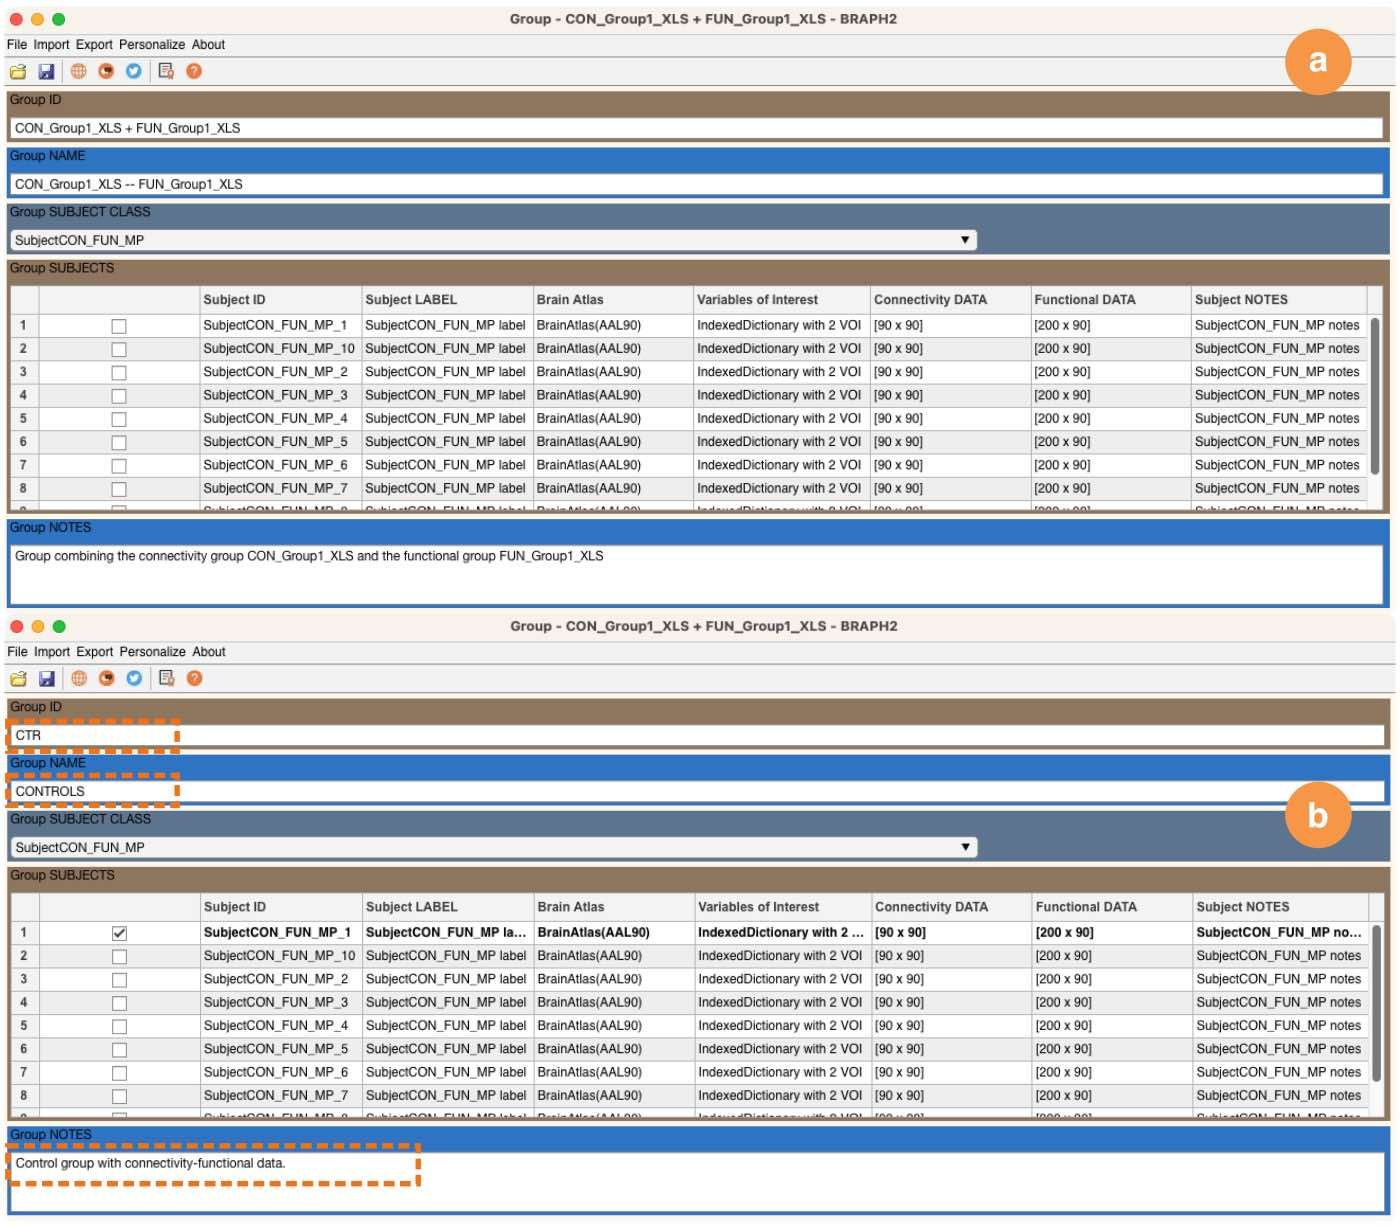
\includegraphics{fig03.jpg}
	}
	{Edit the group metadata}
	{ 
	{\bf a} The GUI of the group's connectivity multiplex data. 
	{\bf b} The information you see on this GUI that can be changed. In this example, we have edited the ID, name, and notes of the group but can also change the subject's specific information.
	}
#!FIG03

\section{Visualize Each Subject's Data}

Finally, you can open each subject's connectivity-functional multiplex data by selecting the subject, right click, and select ''Open selection'' (\Figref{fig:04}a), which shows the matrix values from the connectivity layer and the functional layer (\Figref{fig:04}b). Here, you can also change the subject's metadata (ID, label, notes), its variables of interest, and the values of its connectivity and functional data.

\fig{figure}
	{fig:04}
	{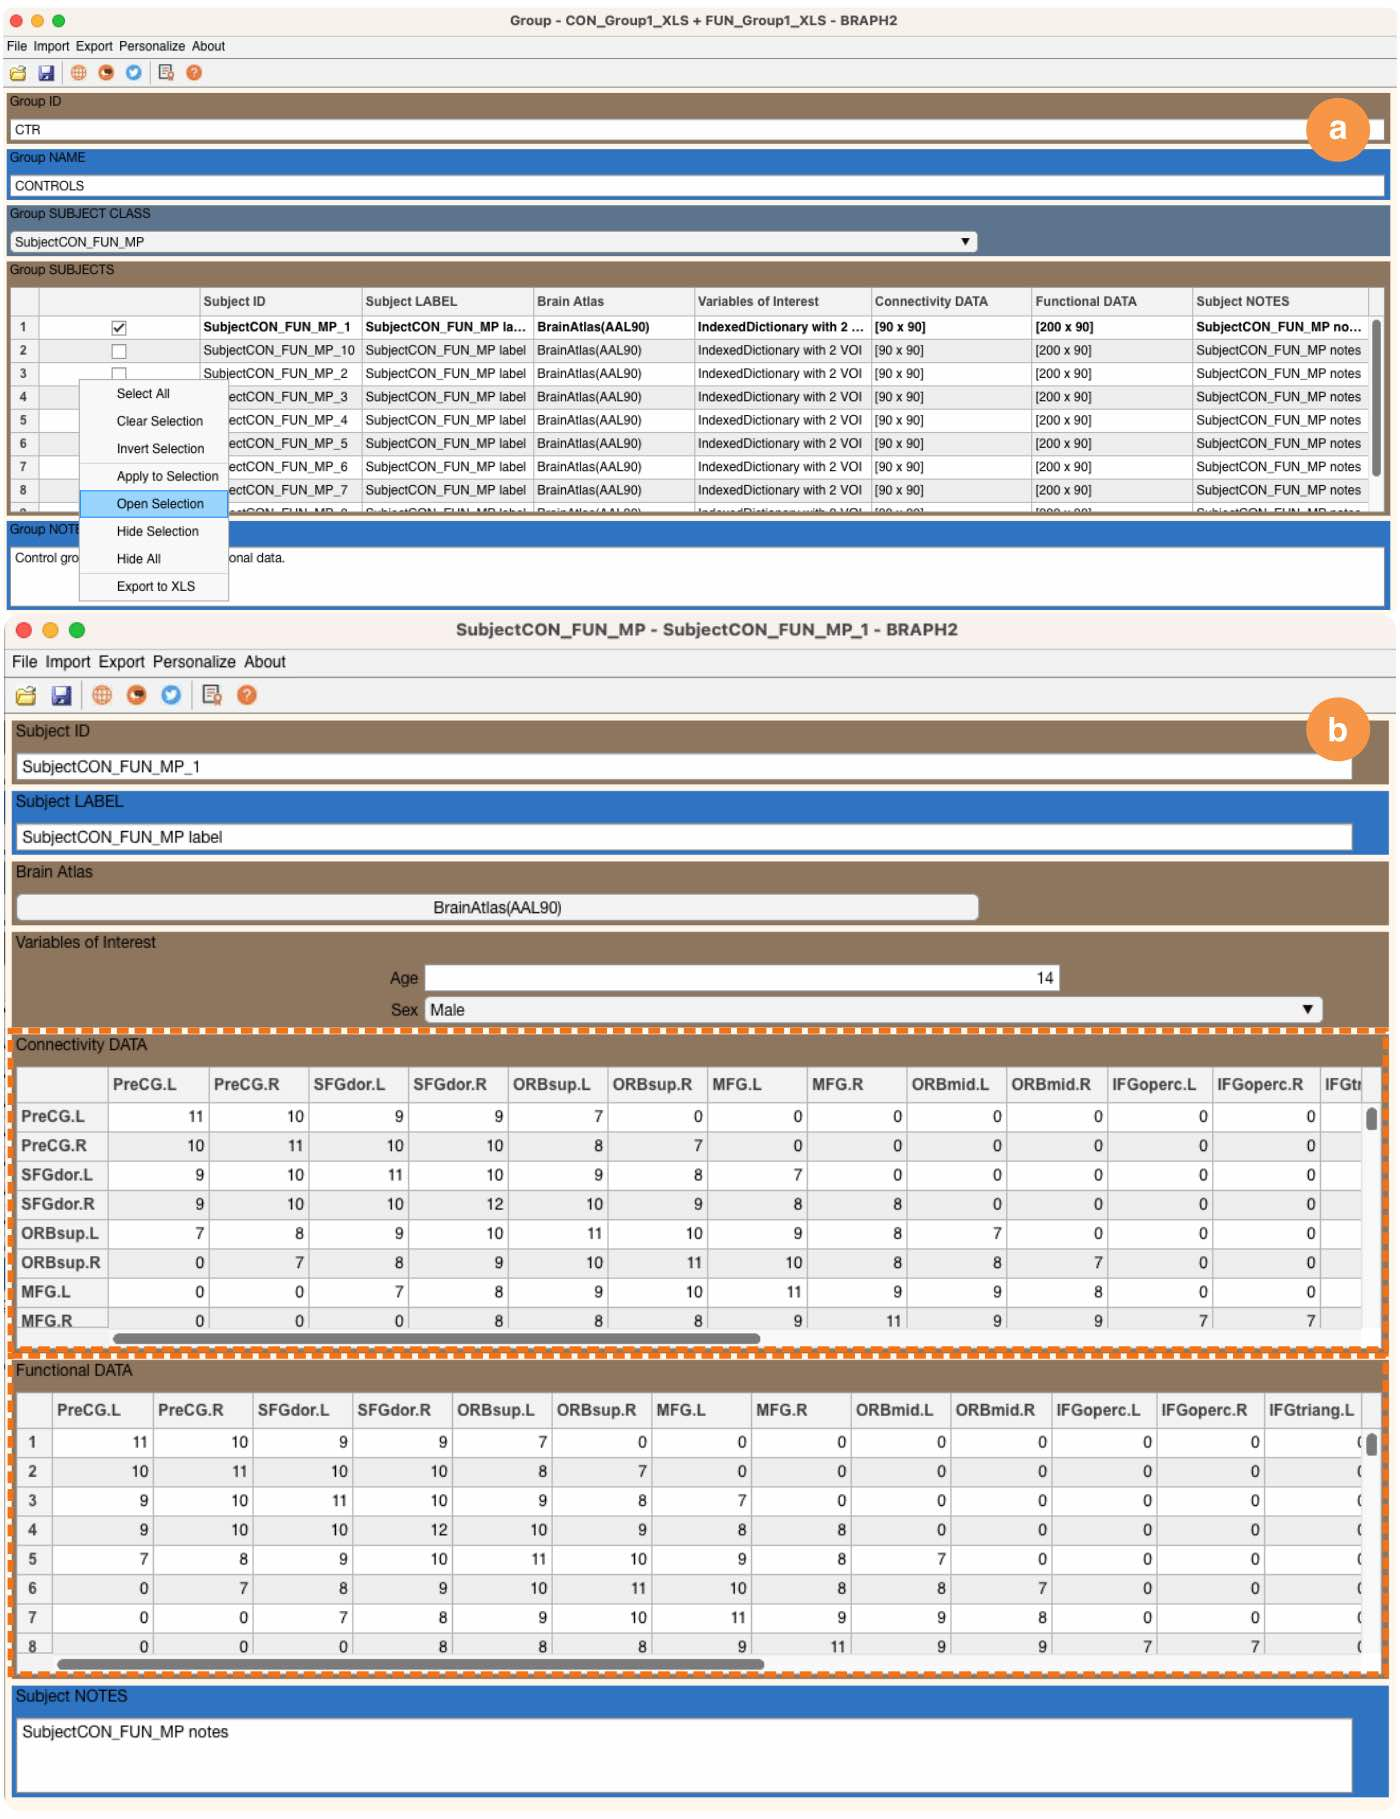
\includegraphics{fig04.jpg}
	}
	{Edit the individual subject data}
	{
	{\bf a}  Each subject's connectivity-functional multiplex data can be opened by selecting the subject, right click, and select ''Open selection''. 
	{\bf b} In this subject GUI, it is possible to view and edit the metadata of the subject (ID, label, notes), its variables of interest (in this case, age and sex), and the connectivity and functional data. 
	}
#!FIG04

\clearpage
\section{Preparation of the Data to be Imported}

To be able to import connectivity-functional multiplex data into BRAPH~2.0, you create a folder with the name of your group, and within this group folder, you need to include a folder for the connectivity data and a folder for the functional data. The organization of the connectivity folder can be checked at the tutorial \href{https://github.com/braph-software/BRAPH-2/tree/develop/tutorials/general/tut_gr_con}{Group of Subjects with Connectivity Data}, and the organization of the functional folder can be check at the tutorial \href{https://github.com/braph-software/BRAPH-2/tree/develop/tutorials/general/tut_gr_fun}{Group of Subjects with Functional Data}. Below in \Figref{fig:05} you can see the directory structure:

\fig{figure*}
	{fig:05}
	{
	[h!]
	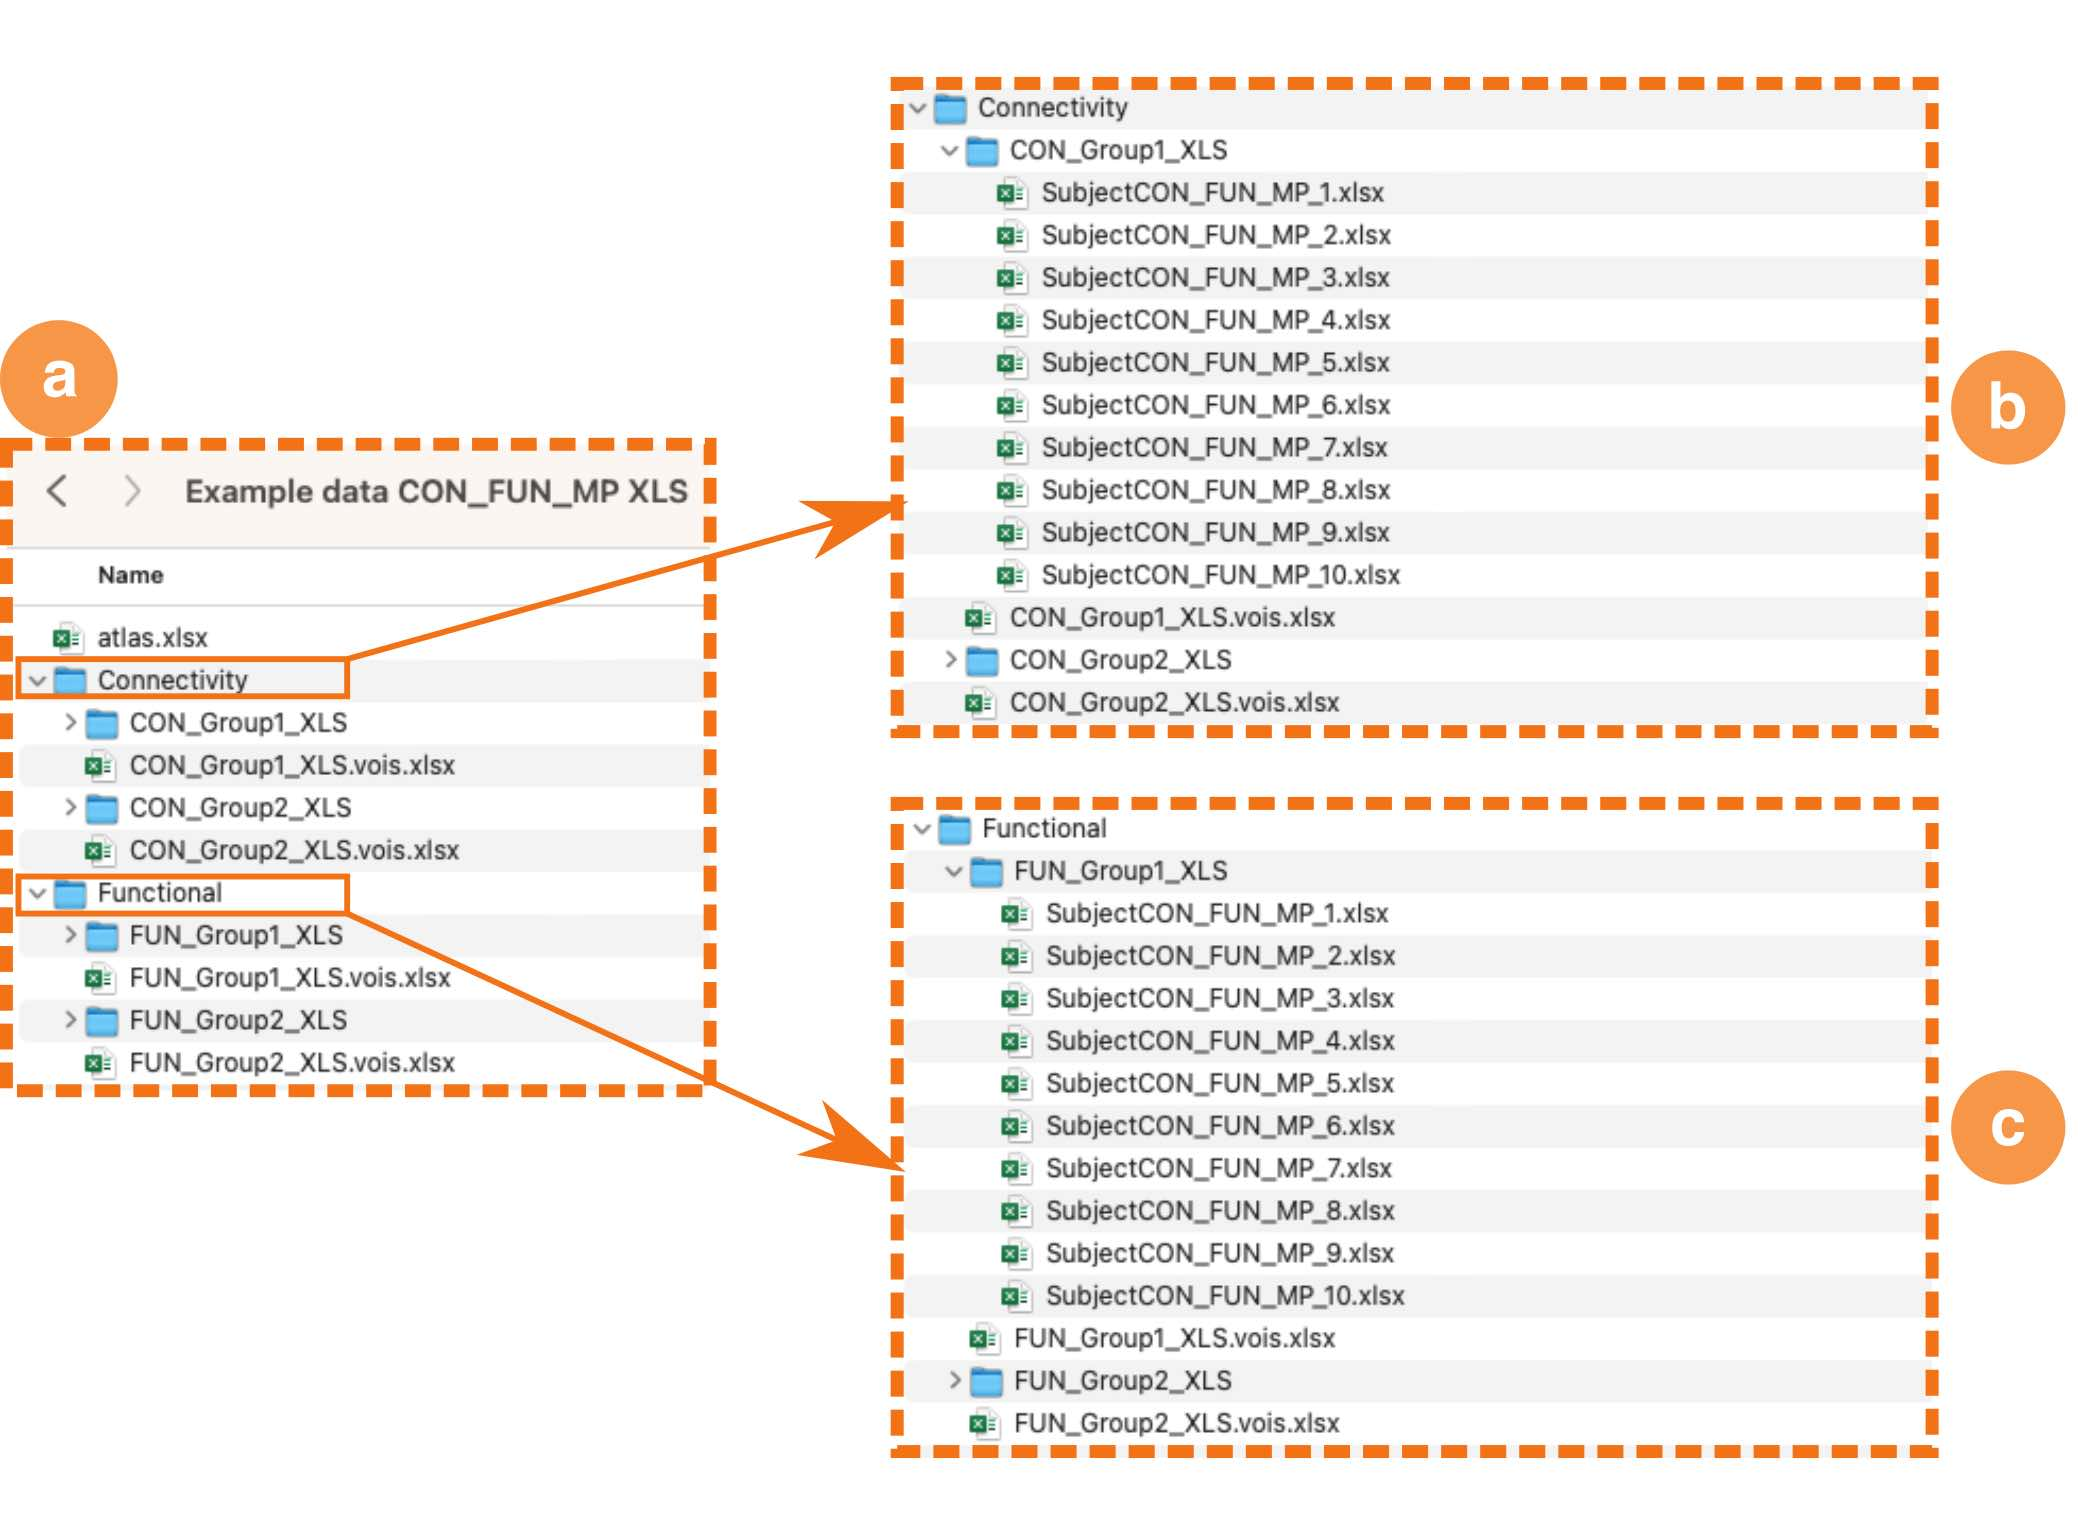
\includegraphics{fig05.jpg}
	}
	{Data preparation}
	{
	The data should be organized in the following format:
	{\bf a} The connectivity matrices from each subject and each layer should be included in one folder (for example, \fn{CON\_MP\_group\_1\_XLS}). 
	{\bf b} Each matrix should contain the connectivity values between each pair of brain regions denoted by the rows and columns. In this example, the (simulated) values in the matrix correspond to the fractional anisotropy (white matter integrity) of anatomical connections derived from diffusion-weighted imaging.
	} 
#!FIG05

\section{Adding Covariates}
	
It is very common to have \emph{variables of interest} (i.e., \emph{covariates} and \emph{correlates}) in an analysis. In BRAPH~2.0, these variables of interest should be included in a separate excel file placed just outside the group's folder and with the same name as the folder followed by \fn{.vois}. It is only necessary to add information to the connectivity folder and not the functional folder if you want to include covariates; however, if you already have the information in the functional folder, there won’t be any issues.
This file should have a specific format:
\begin{itemize}

\item[Subject IDs (column A).]
Column A should contain the subject IDs starting from row 3.

\item[Variables of interest (column B and subsequent columns).]
Column B (and subsequent columns) should contain the variables of interest (one per column). 
In this example we have ``Age'' and ``Sex'', as in the example file, as well as the additional ``Education''.
In each column, row 1 should contain the name of the variable of interest, row 2 should contain the categories separated by a return (only for categorical variables of interest, like ``Sex'' and ``Education''), and the subsequent rows the values of the variable of interest for each subject.

\end{itemize}	

\end{document}